\documentclass[10pt]{beamer}

\usepackage[UTF8,noindent]{ctex}
\usepackage{times}
\usepackage{fontenc}
\usetheme{Singapore}
\setbeamertemplate{navigation symbols}{}
\setbeamertemplate{background}{
\includegraphics[height=\paperheight]{bg}}
\title[中期答辩]{“卷皮网”用户画像及精准推荐实战}
\subtitle{大学生创新训练项目中期答辩}
\author[用户画像与机器学习实战]{答辩人:孙嘉轩\ 黄爽\ 龙海文\ 杨岳浩\ 许艳\newline \newline 指导老师:张千帆}
\institute[]{华中科技大学管理学院}

%%%%%%%%%%%%%%%%%%%%%%%%%%%%%%%%%%
\begin{document}
%%%%%%%%%%%%%%%%%%%%%%%%%%%%%%%%%%

\frame{\titlepage}
\begin{frame}
\textbf{"There is nothing about doing data analysis that is neutral.\newline
What and how data is collected, how the data is cleaned\newline and
stored, what models are constructed, and what questions are
asked – all of this is political."}
\newline Danah Boyd, NYU

\end{frame}

\begin{frame}{Outline}
\tableofcontents
\end{frame}

\section{项目进展}

\begin{frame}{企业合作}
  \begin{itemize}
  \item 与卷皮网员工进行交流
  \newline
  \item 爬取并分析卷皮网相关数据
  \newline
  \item 发现数据潜在商业价值与市场应用
  \end{itemize}
\end{frame}

%%%%%%

\begin{frame}{网页}
\begin{columns}
  \begin{column}{0.4\textwidth}
    \textbf{userprofileguide.github.io}
  \end{column}
  \begin{column}{0.6\textwidth}
    
\includegraphics[height=0.4\paperheight]{website1}
    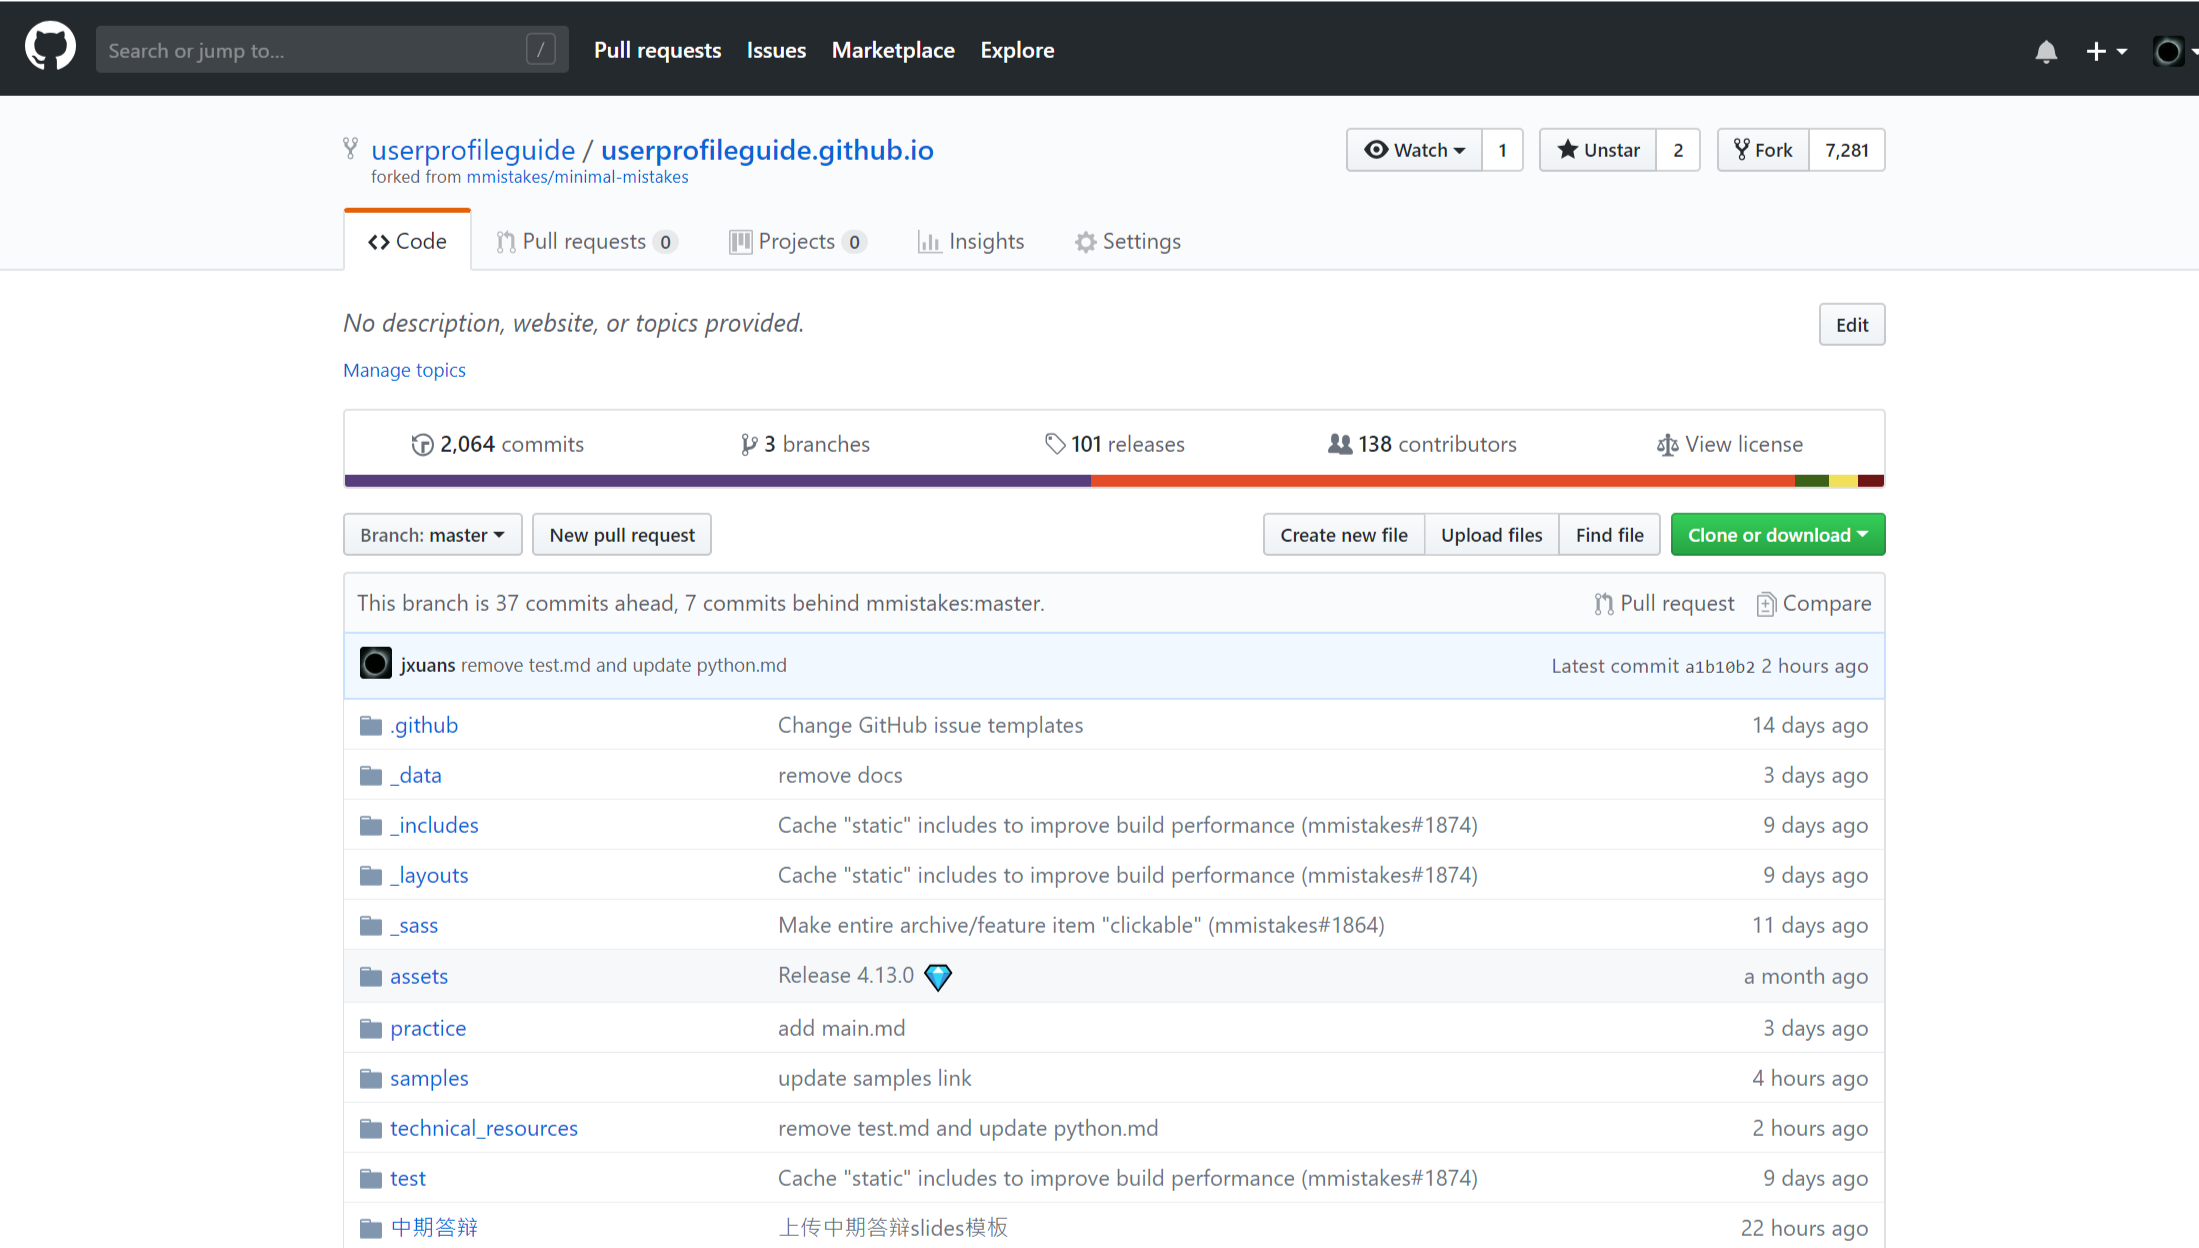
\includegraphics[height=0.4\paperheight]{website2}
  \end{column}
  \end{columns}
\end{frame}

%%%%%%

\section{现阶段问题}
  \begin{frame}{现阶段问题}

  \end{frame}

%%%%%%

\section{财务情况}
  \begin{frame}{ }
  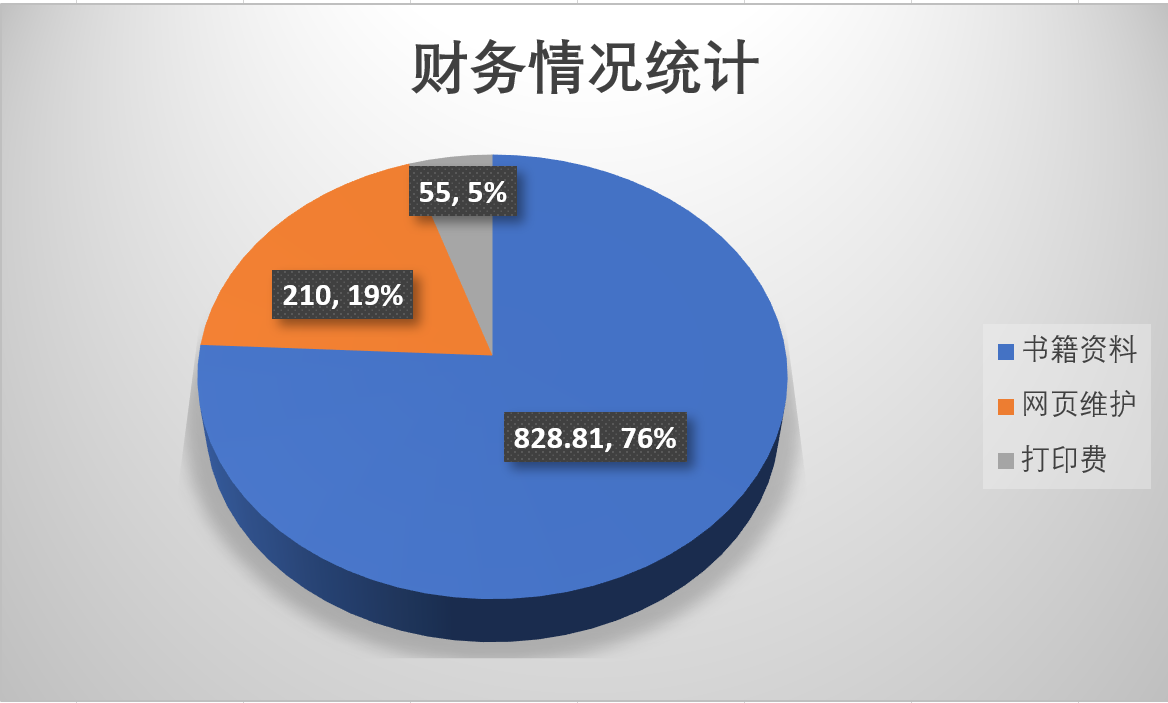
\includegraphics[height=0.66\paperheight]{finance}
  \end{frame}

%%%%%%

\section{后续工作安排}
  \begin{frame}{后续工作安排}

  \end{frame}


%%%%%%


\begin{frame}
\textbf{Thank you for listening!}
\end{frame}

\end{document}
